%% main.tex
%% V1.3
%% 2007/01/11
%% by Michael Shell
%% See:
%% http://www.michaelshell.org/
%% for current contact information.
%%
%% This is a skeleton file demonstrating the use of IEEEtran.cls
%% (requires IEEEtran.cls version 1.7 or later) with an IEEE conference paper.
%%
%% Support sites:
%% http://www.michaelshell.org/tex/ieeetran/
%% http://www.ctan.org/tex-archive/macros/latex/contrib/IEEEtran/
%% and
%% http://www.ieee.org/

%%*************************************************************************
%% Legal Notice:
%% This code is offered as-is without any warranty either expressed or
%% implied; without even the implied warranty of MERCHANTABILITY or
%% FITNESS FOR A PARTICULAR PURPOSE! 
%% User assumes all risk.
%% In no event shall IEEE or any contributor to this code be liable for
%% any damages or losses, including, but not limited to, incidental,
%% consequential, or any other damages, resulting from the use or misuse
%% of any information contained here.
%%
%% All comments are the opinions of their respective authors and are not
%% necessarily endorsed by the IEEE.
%%
%% This work is distributed under the LaTeX Project Public License (LPPL)
%% ( http://www.latex-project.org/ ) version 1.3, and may be freely used,
%% distributed and modified. A copy of the LPPL, version 1.3, is included
%% in the base LaTeX documentation of all distributions of LaTeX released
%% 2003/12/01 or later.
%% Retain all contribution notices and credits.
%% ** Modified files should be clearly indicated as such, including  **
%% ** renaming them and changing author support contact information. **
%%
%% File list of work: IEEEtran.cls, IEEEtran_HOWTO.pdf, bare_adv.tex,
%%                    bare_conf.tex, bare_jrnl.tex, bare_jrnl_compsoc.tex
%%*************************************************************************

% *** Authors should verify (and, if needed, correct) their LaTeX system  ***
% *** with the testflow diagnostic prior to trusting their LaTeX platform ***
% *** with production work. IEEE's font choices can trigger bugs that do  ***
% *** not appear when using other class files.                            ***
% The testflow support page is at:
% http://www.michaelshell.org/tex/testflow/



% Note that the a4paper option is mainly intended so that authors in
% countries using A4 can easily print to A4 and see how their papers will
% look in print - the typesetting of the document will not typically be
% affected with changes in paper size (but the bottom and side margins will).
% Use the testflow package mentioned above to verify correct handling of
% both paper sizes by the user's LaTeX system.
%
% Also note that the "draftcls" or "draftclsnofoot", not "draft", option
% should be used if it is desired that the figures are to be displayed in
% draft mode.
%
\documentclass[10pt, conference, compsocconf]{IEEEtran}
% Add the compsocconf option for Computer Society conferences.
%
% If IEEEtran.cls has not been installed into the LaTeX system files,
% manually specify the path to it like:
% \documentclass[conference]{../sty/IEEEtran}





% Some very useful LaTeX packages include:
% (uncomment the ones you want to load)


% *** MISC UTILITY PACKAGES ***
%
%\usepackage{ifpdf}
% Heiko Oberdiek's ifpdf.sty is very useful if you need conditional
% compilation based on whether the output is pdf or dvi.
% usage:
% \ifpdf
%   % pdf code
% \else
%   % dvi code
% \fi
% The latest version of ifpdf.sty can be obtained from:
% http://www.ctan.org/tex-archive/macros/latex/contrib/oberdiek/
% Also, note that IEEEtran.cls V1.7 and later provides a builtin
% \ifCLASSINFOpdf conditional that works the same way.
% When switching from latex to pdflatex and vice-versa, the compiler may
% have to be run twice to clear warning/error messages.






% *** CITATION PACKAGES ***
%
%\usepackage{cite}
% cite.sty was written by Donald Arseneau
% V1.6 and later of IEEEtran pre-defines the format of the cite.sty package
% \cite{} output to follow that of IEEE. Loading the cite package will
% result in citation numbers being automatically sorted and properly
% "compressed/ranged". e.g., [1], [9], [2], [7], [5], [6] without using
% cite.sty will become [1], [2], [5]--[7], [9] using cite.sty. cite.sty's
% \cite will automatically add leading space, if needed. Use cite.sty's
% noadjust option (cite.sty V3.8 and later) if you want to turn this off.
% cite.sty is already installed on most LaTeX systems. Be sure and use
% version 4.0 (2003-05-27) and later if using hyperref.sty. cite.sty does
% not currently provide for hyperlinked citations.
% The latest version can be obtained at:
% http://www.ctan.org/tex-archive/macros/latex/contrib/cite/
% The documentation is contained in the cite.sty file itself.






% *** GRAPHICS RELATED PACKAGES ***
%
\ifCLASSINFOpdf
  % \usepackage[pdftex]{graphicx}
  % declare the path(s) where your graphic files are
  % \graphicspath{{../pdf/}{../jpeg/}}
  % and their extensions so you won't have to specify these with
  % every instance of \includegraphics
  % \DeclareGraphicsExtensions{.pdf,.jpeg,.png}
\else
  % or other class option (dvipsone, dvipdf, if not using dvips). graphicx
  % will default to the driver specified in the system graphics.cfg if no
  % driver is specified.
  % \usepackage[dvips]{graphicx}
  % declare the path(s) where your graphic files are
  % \graphicspath{{../eps/}}
  % and their extensions so you won't have to specify these with
  % every instance of \includegraphics
  % \DeclareGraphicsExtensions{.eps}
\fi
% graphicx was written by David Carlisle and Sebastian Rahtz. It is
% required if you want graphics, photos, etc. graphicx.sty is already
% installed on most LaTeX systems. The latest version and documentation can
% be obtained at: 
% http://www.ctan.org/tex-archive/macros/latex/required/graphics/
% Another good source of documentation is "Using Imported Graphics in
% LaTeX2e" by Keith Reckdahl which can be found as epslatex.ps or
% epslatex.pdf at: http://www.ctan.org/tex-archive/info/
%
% latex, and pdflatex in dvi mode, support graphics in encapsulated
% postscript (.eps) format. pdflatex in pdf mode supports graphics
% in .pdf, .jpeg, .png and .mps (metapost) formats. Users should ensure
% that all non-photo figures use a vector format (.eps, .pdf, .mps) and
% not a bitmapped formats (.jpeg, .png). IEEE frowns on bitmapped formats
% which can result in "jaggedy"/blurry rendering of lines and letters as
% well as large increases in file sizes.
%
% You can find documentation about the pdfTeX application at:
% http://www.tug.org/applications/pdftex





% *** MATH PACKAGES ***
%
%\usepackage[cmex10]{amsmath}
% A popular package from the American Mathematical Society that provides
% many useful and powerful commands for dealing with mathematics. If using
% it, be sure to load this package with the cmex10 option to ensure that
% only type 1 fonts will utilized at all point sizes. Without this option,
% it is possible that some math symbols, particularly those within
% footnotes, will be rendered in bitmap form which will result in a
% document that can not be IEEE Xplore compliant!
%
% Also, note that the amsmath package sets \interdisplaylinepenalty to 10000
% thus preventing page breaks from occurring within multiline equations. Use:
%\interdisplaylinepenalty=2500
% after loading amsmath to restore such page breaks as IEEEtran.cls normally
% does. amsmath.sty is already installed on most LaTeX systems. The latest
% version and documentation can be obtained at:
% http://www.ctan.org/tex-archive/macros/latex/required/amslatex/math/





% *** SPECIALIZED LIST PACKAGES ***
%
%\usepackage{algorithmic}
% algorithmic.sty was written by Peter Williams and Rogerio Brito.
% This package provides an algorithmic environment fo describing algorithms.
% You can use the algorithmic environment in-text or within a figure
% environment to provide for a floating algorithm. Do NOT use the algorithm
% floating environment provided by algorithm.sty (by the same authors) or
% algorithm2e.sty (by Christophe Fiorio) as IEEE does not use dedicated
% algorithm float types and packages that provide these will not provide
% correct IEEE style captions. The latest version and documentation of
% algorithmic.sty can be obtained at:
% http://www.ctan.org/tex-archive/macros/latex/contrib/algorithms/
% There is also a support site at:
% http://algorithms.berlios.de/index.html
% Also of interest may be the (relatively newer and more customizable)
% algorithmicx.sty package by Szasz Janos:
% http://www.ctan.org/tex-archive/macros/latex/contrib/algorithmicx/




% *** ALIGNMENT PACKAGES ***
%
%\usepackage{array}
% Frank Mittelbach's and David Carlisle's array.sty patches and improves
% the standard LaTeX2e array and tabular environments to provide better
% appearance and additional user controls. As the default LaTeX2e table
% generation code is lacking to the point of almost being broken with
% respect to the quality of the end results, all users are strongly
% advised to use an enhanced (at the very least that provided by array.sty)
% set of table tools. array.sty is already installed on most systems. The
% latest version and documentation can be obtained at:
% http://www.ctan.org/tex-archive/macros/latex/required/tools/


%\usepackage{mdwmath}
%\usepackage{mdwtab}
% Also highly recommended is Mark Wooding's extremely powerful MDW tools,
% especially mdwmath.sty and mdwtab.sty which are used to format equations
% and tables, respectively. The MDWtools set is already installed on most
% LaTeX systems. The lastest version and documentation is available at:
% http://www.ctan.org/tex-archive/macros/latex/contrib/mdwtools/


% IEEEtran contains the IEEEeqnarray family of commands that can be used to
% generate multiline equations as well as matrices, tables, etc., of high
% quality.


%\usepackage{eqparbox}
% Also of notable interest is Scott Pakin's eqparbox package for creating
% (automatically sized) equal width boxes - aka "natural width parboxes".
% Available at:
% http://www.ctan.org/tex-archive/macros/latex/contrib/eqparbox/





% *** SUBFIGURE PACKAGES ***
%\usepackage[tight,footnotesize]{subfigure}
% subfigure.sty was written by Steven Douglas Cochran. This package makes it
% easy to put subfigures in your figures. e.g., "Figure 1a and 1b". For IEEE
% work, it is a good idea to load it with the tight package option to reduce
% the amount of white space around the subfigures. subfigure.sty is already
% installed on most LaTeX systems. The latest version and documentation can
% be obtained at:
% http://www.ctan.org/tex-archive/obsolete/macros/latex/contrib/subfigure/
% subfigure.sty has been superceeded by subfig.sty.



%\usepackage[caption=false]{caption}
%\usepackage[font=footnotesize]{subfig}
% subfig.sty, also written by Steven Douglas Cochran, is the modern
% replacement for subfigure.sty. However, subfig.sty requires and
% automatically loads Axel Sommerfeldt's caption.sty which will override
% IEEEtran.cls handling of captions and this will result in nonIEEE style
% figure/table captions. To prevent this problem, be sure and preload
% caption.sty with its "caption=false" package option. This is will preserve
% IEEEtran.cls handing of captions. Version 1.3 (2005/06/28) and later 
% (recommended due to many improvements over 1.2) of subfig.sty supports
% the caption=false option directly:
%\usepackage[caption=false,font=footnotesize]{subfig}
%
% The latest version and documentation can be obtained at:
% http://www.ctan.org/tex-archive/macros/latex/contrib/subfig/
% The latest version and documentation of caption.sty can be obtained at:
% http://www.ctan.org/tex-archive/macros/latex/contrib/caption/




% *** FLOAT PACKAGES ***
%
%\usepackage{fixltx2e}
% fixltx2e, the successor to the earlier fix2col.sty, was written by
% Frank Mittelbach and David Carlisle. This package corrects a few problems
% in the LaTeX2e kernel, the most notable of which is that in current
% LaTeX2e releases, the ordering of single and double column floats is not
% guaranteed to be preserved. Thus, an unpatched LaTeX2e can allow a
% single column figure to be placed prior to an earlier double column
% figure. The latest version and documentation can be found at:
% http://www.ctan.org/tex-archive/macros/latex/base/



%\usepackage{stfloats}
% stfloats.sty was written by Sigitas Tolusis. This package gives LaTeX2e
% the ability to do double column floats at the bottom of the page as well
% as the top. (e.g., "\begin{figure*}[!b]" is not normally possible in
% LaTeX2e). It also provides a command:
%\fnbelowfloat
% to enable the placement of footnotes below bottom floats (the standard
% LaTeX2e kernel puts them above bottom floats). This is an invasive package
% which rewrites many portions of the LaTeX2e float routines. It may not work
% with other packages that modify the LaTeX2e float routines. The latest
% version and documentation can be obtained at:
% http://www.ctan.org/tex-archive/macros/latex/contrib/sttools/
% Documentation is contained in the stfloats.sty comments as well as in the
% presfull.pdf file. Do not use the stfloats baselinefloat ability as IEEE
% does not allow \baselineskip to stretch. Authors submitting work to the
% IEEE should note that IEEE rarely uses double column equations and
% that authors should try to avoid such use. Do not be tempted to use the
% cuted.sty or midfloat.sty packages (also by Sigitas Tolusis) as IEEE does
% not format its papers in such ways.





% *** PDF, URL AND HYPERLINK PACKAGES ***
%
%\usepackage{url}
% url.sty was written by Donald Arseneau. It provides better support for
% handling and breaking URLs. url.sty is already installed on most LaTeX
% systems. The latest version can be obtained at:
% http://www.ctan.org/tex-archive/macros/latex/contrib/misc/
% Read the url.sty source comments for usage information. Basically,
% \url{my_url_here}.





% *** Do not adjust lengths that control margins, column widths, etc. ***
% *** Do not use packages that alter fonts (such as pslatex).         ***
% There should be no need to do such things with IEEEtran.cls V1.6 and later.
% (Unless specifically asked to do so by the journal or conference you plan
% to submit to, of course. )


% correct bad hyphenation here
\hyphenation{op-tical net-works semi-conduc-tor}



\usepackage{graphicx}
% \usepackage{enumerate}
\usepackage{amsmath}

\usepackage{subcaption}
\usepackage{tikz}
\usepackage{longtable}
\usepackage[english]{babel}
\usepackage{setspace}
\usepackage{algorithm}
\usepackage[noend]{algpseudocode}
\usepackage{changepage}
\usepackage{amssymb}

% \usepackage{tabulary}

\usepackage{listings}
\usepackage{float}









\begin{document}
%
% paper title
% can use linebreaks \\ within to get better formatting as desired
\title{Exploring Power-Performance-Quality trade-offs for Exascale Combustion Simulation}


% author names and affiliations
% use a multiple column layout for up to two different
% affiliations

\author{\IEEEauthorblockN{Authors Name/s per 1st Affiliation (Author)}
\IEEEauthorblockA{line 1 (of Affiliation): dept. name of organization\\
line 2: name of organization, acronyms acceptable\\
line 3: City, Country\\
line 4: Email: name@xyz.com}
\and
\IEEEauthorblockN{Authors Name/s per 2nd Affiliation (Author)}
\IEEEauthorblockA{line 1 (of Affiliation): dept. name of organization\\
line 2: name of organization, acronyms acceptable\\
line 3: City, Country\\
line 4: Email: name@xyz.com}
}

% conference papers do not typically use \thanks and this command
% is locked out in conference mode. If really needed, such as for
% the acknowledgment of grants, issue a \IEEEoverridecommandlockouts
% after \documentclass

% for over three affiliations, or if they all won't fit within the width
% of the page, use this alternative format:
% 
%\author{\IEEEauthorblockN{Michael Shell\IEEEauthorrefmark{1},
%Homer Simpson\IEEEauthorrefmark{2},
%James Kirk\IEEEauthorrefmark{3}, 
%Montgomery Scott\IEEEauthorrefmark{3} and
%Eldon Tyrell\IEEEauthorrefmark{4}}
%\IEEEauthorblockA{\IEEEauthorrefmark{1}School of Electrical and Computer Engineering\\
%Georgia Institute of Technology,
%Atlanta, Georgia 30332--0250\\ Email: see http://www.michaelshell.org/contact.html}
%\IEEEauthorblockA{\IEEEauthorrefmark{2}Twentieth Century Fox, Springfield, USA\\
%Email: homer@thesimpsons.com}
%\IEEEauthorblockA{\IEEEauthorrefmark{3}Starfleet Academy, San Francisco, California 96678-2391\\
%Telephone: (800) 555--1212, Fax: (888) 555--1212}
%\IEEEauthorblockA{\IEEEauthorrefmark{4}Tyrell Inc., 123 Replicant Street, Los Angeles, California 90210--4321}}




% use for special paper notices
%\IEEEspecialpapernotice{(Invited Paper)}




% make the title area
\maketitle


\begin{abstract}
The computational demand of high-performance computing (HPC) applications has brought major changes to the HPC system architecture. As a result, it is now possible to run simulations faster and get more accurate results. But behind this, power and energy are becoming critical concerns for HPC systems, e.g. Titan’s electric cost is about \$9 million per year\cite{computerworld}. Power efficiency has become a critical challenge for the exascale research challenges, and U.S. Department of Energy (DOE) has set the goal to achieve exascale performance with a power budget of 20MW\cite{lucas2014doe}.

Current research efforts have studied power and performance tradeoffs, and how to balance these, e.g., using DVFS to meet power constraints, which significantly impacts performance. However, scientific applications may not tolerate degradation in performance and other tradeoffs need to be explored to meet power budgets, e.g., involving the application in making energy-performance tradeoff decisions. 

This research focuses on studying the properties and exploring the performance and power\/energy tradeoffs of Low-Mach-Number Combustion (LMC) application which is an Adaptive Mesh Refinement (AMR) algorithm. Our experimental evaluation provides an empirical evaluation of different application configurations that gives insights into the power-performance tradeoffs space for this LMC or AMR-based application workflows. The key contribution of this work is a better understanding of the running behavior of this AMR-based application and the power-performance tradeoffs for this application under power constraints, which can be used to better schedule power budgets across HPC systems.

\end{abstract}

\begin{IEEEkeywords}
Power-Performance-Quality, trade-offs, Exascale

\end{IEEEkeywords}


% For peer review papers, you can put extra information on the cover
% page as needed:
% \ifCLASSOPTIONpeerreview
% \begin{center} \bfseries EDICS Category: 3-BBND \end{center}
% \fi
%
% For peerreview papers, this IEEEtran command inserts a page break and
% creates the second title. It will be ignored for other modes.
\IEEEpeerreviewmaketitle



\section{Introduction}
% no \IEEEPARstart

High performance computing (HPC) have been played an important role in the field of computational science in 21st century. However,as we are approaching the exascale era, power is turning from an optimization goal to a critical operation constraint. U.S Department of Energy (DOE) has currently set a bound of 20MW for an exascale system.\cite{tolentino2012optimist} This strict power constraint poses a hard research challenge with current hardware and software. 

In order to achieve this exascale system power constraint, many research efforts have studied power and performance tradeoffs, and most energy models or strategies are based on runtime (e.g., leveraging MPI slack) for power clamping or power capping techniques, like Dynamic Voltage and Frequency Scaling (DVFS) to constraint the power. However, power and performance are in the two sides of a balance scale, that it is hard to improve one side without scarifying the other one. Therefore, one of the key problems addressed in this research is keeping the power bound (or budget) without losing performance, which is challenging for real world application targeting exascale.

To address this challenge, we believe that the applications should be involved in making tradeoff decisions. This research targets a Center for Exascale simulation of Combustion in Turbulence (ExaCT) Low-Mach-number Combustion simulation code (LMC). \cite{exact} This combustion simulation is developed based on Adaptive-Mesh-Refinement (AMR) algorithm. The AMR method can be customized to resolve problems at different resolution levels. This property motivates us to find the potential tradeoffs to run applications in power-constrained environments without impacting performance by tolerating lower resolution/quality levels, together with power capping.

The contribution of this work are 1) present an empirical evaluation of different configurations of application that gives insights into the energy-performance-quality tradeoff for scientific data-driven workflows. 2) provide a comprehensive study of this LMC simulation performance, quality, and power and energy behavior. 3) present a proof-of-concept study of potential of power capping and power management to balance power-performance-quality tradeoffs.

The rest of this paper is organized as follows. Chapter 2 summarizes the related work. Chapter 3 presents background information related to the techniques used in this research. Chapter 4 describes the evaluation methodology and presents the results of the experimental evaluation. Chapter 5 concludes the chapter and outlines ongoing and future research.



\section{Related works}
\subsection{Energy efficiency}
Energy-efficiency has become a critical concern for HPC applications. There are many approaches have been proposed to obtaining energy savings during HPC application execution. Some of them are to focus on identifying stalls during the execution by measuring architectural parameters from performance counters as proposed in\cite{ge2007cpu,hsu2005power,huang2009energy}. In addition to using performance counters, Rountree et al.\cite{rountree2009adagio} developed a runtime system called Adagio, by doing the critical path analysis, it can determine which tasks may be slowed down and also suitable opportunities to apply DVFS to minimize the performance loss in the parallel execution. This achieves significant energy saving in scientific application with negligible performance lose. However, this approach appears beneficial when applications have computation or communication imbalances among participating processes, which is typically not the case for a highly efficient parallel application nor suitable for the LMC program targeted in this work. Some approaches in\cite{freeh2005using,lim2006adaptive} are proposing to determine the communication phases to apply DVFS. Kandalla et al.\cite{kandalla2010designing} give algorithms to save energy in the collectives such as MPI\_Alltoall and MPI\_Bcase. Moreover, Ioannou et al.\cite{ioannou2011phase} describe a runtime system for the Intel Single-chip Cloud Computer (SCC) processor to detect repeatable communication phases followed by an application of frequency scaling. Donofrio et al.\cite{donofrio2009energy} have studied energy efficiency for extreme-scale science and developed Green Flash, an application-driven design to improve the kernel’s computational efficiency. Li et al.\cite{li2010hybrid} developed a new power-aware performance prediction model of hybrid MPI/OpenMP programming model and combine memory and disk management techniques to provide performance guarantees for control algorithms. Rodero et al.\cite{rodero2010investigating} explored the potential of application-centric aggressive power management of HPC scientific workloads while considering power management mechanisms and controls available at different levels and different subsystems. Gmall et al.\cite{gamell2013exploring} explored data-related energy/performance trade-offs for end-to-end co-design simulation workflows on current and on-going high-end computing systems. Lively et al.\cite{lively2011energy} explored and investigated energy consumption and execution time of different parallel implementation of scientific applications on multi-cluster systems. 

Most of the work described above are from system level and are based on tolerating performance loss and constrain the power consumption under that performance loss. The work presented here discusses the possibility to filter down power constraint to job-level, and then take advantage of applications specific properties, such as resolution, to keep the power budget while maintaining the level of performance. 

\subsection{Power management}
The cost of provisioning power in data centers is a very large fraction of the total cost of operating a data center.\cite{pelley2010power,hamilton2008cost} Therefore the ability to cap peak power consumption is a desirable feature in modern data centers.\cite{cochran2011pack} Many power management approaches have been proposed to provide performance guarantees while constraining power budget. Sartori et al.\cite{sartori2009distributed} describe a peak power management technique for multi-core systems by choosing the power state for each core that meets the power constraints. Cebrian et al.\cite{cebrian2011power} develop a power balancing strategy that through borrowing power budgets from cores that consume lower power to dynamically adapts the per-core power budgets. While, Gandhi et al.\cite{gandhi2009power} give a power capping strategy to meet the power budget by inserting idle cycles during execution. This approach aims at controlling the average power consumption, but cannot guarantee the peak power. So a number of other approaches are proposed through reconfiguring hardware to meet the power budget. Meng et al.\cite{meng2008multi} provide a power management strategy through dynamic reconfiguration of cores by cache resizing. Konotorinis et al.\cite{kontorinis2009reducing} propose a table-driven adaptive core reconfiguration technique that configures core resources such as load-store queues and floating point units to meet peak power budget. Most of the power management strategies are using DVFS. Since Intel SandyBridge family processors, Intel provide Running Average Power Limit (RAPL) for controlling the power constraint on processors and memory. Several studies have begun to evaluate the RAPL power management system. Rountree et al.\cite{rountree2012beyond} explore RAPL as a replacement for DVFS in HPC systems by evaluating power consumption for package and memory subsystem. Zhang et al.\cite{zhang2015quantitative} give a systematic evaluation of RAPL behavior such as stability, setting time, overshoot and, etc. RAPL also been used to study application runtime variability and power optimization for exascale computing in work of Allan et al.\cite{porterfield2015application}[21] Sarood et al.\cite{sarood2013optimizing} use RAPL to set power bounds on across an over-provisioned cluster running homogeneous application processes.  This work also takes advantage of RAPL power controlling ability to dynamically manage power consumption.



\subsection{Power measurement systems}
Measuring the power/energy consumption of software components is the key for energy-aware scheduling, accounting and budgeting. RAPL measurement mechanism is described in\cite{porterfield2015application} and Marcus et al.\cite{hahnel2012measuring} has investigated the RAPL measurements performance and discussed the practical obstacles that existed in performing these measurements on complex modern CPUs. Vignesh et al.\cite{adhinarayanan2015greenness} studied the greenness of the in-situ and the post-processing visualization pipelines using RAPL to measure the CPUs and RAMs power consumption and with an average error rate of less than 1\%. Venkatesh et al.\cite{venkatesh2013evaluation} use RAPL to measure energy consumption in large message-passing applications.


\section{Experimental evaluation}
\subsection{Infrastructure overviews}
\subsubsection{CAPER Cluster}
CAPER (Computational And data-enabled Platform for Energy efficiency Research) is a unique and flexible instrument funded by The National Science Foundation that combines high performance Intel Xeon processors with a complete deep memory hierarchy, latest generation co-processors, high performance network interconnect and powerful system power instrumentation.

It is currently an eight-node cluster, which is capable of housing concurrently, in one node up to eight general-purpose graphical processing units (GPGPU), or eight Intel many-integrated-core (MIC) coprocessors - or any eight-card combination of the two; and up to 48 hard disk drives (HDD), or solid-state drives (SSD). A single-node configuration features a theoretical peak performance of 20TF/s (single precisions) or 10TF/s (double precision) and supports up to 32TB of storage and 24TB of flash-based non-volatile memory. A separate node serves as a login and storage server.

This hardware configuration is unprecedented in its flexibility and adaptability as it can combine multiple components into a smaller set of nodes to reproduce specific configurations. This platform also mirrors key architectural characteristics of high-end system, such as XSEDE's Stampede system at TACC, and provides several unique features to support critical research goals such as software/hardware co-design. CAPER provides a platform to validate models and investigate important aspects of data-centric and energy efficiency research.


\subsubsection{DELL Cluster}
DELL platform includes a 32 node Dell M610 blade cluster, consisting of two Dell M1000E Modular Blade Enclosures, necessary interconnect/management infrastructure, and a supervisory node. Each enclosure is maximally configured with sixteen blades, each blade having two Intel Xeon E5504 Nehalem family quad-core processors at 2.0 GHz, forming an eight core node. Each node has 24 GB RAM and 73 GB of local disk storage (10,000 RPM), twelve nodes have an additional 1 TB of local storage. The network infrastructure is comprised of an integrated 16-port Mellanox InfiniBand switch within each blade chassis, each switch linked to the switch in the other chassis. All blades have Mellanox Quad-Data-Rate (QDR) InfiniBand interface cards. There is also an integrated (redundant) 1 Gigabit Ethernet within each chassis, with two pairs of 10 Gigabit uplink capabilities in each chassis. In the aggregate, the cluster system consists of 32 nodes, 256 cores, 768 GB memory and ~14.5 TB disk capacity, with a 20 Gigabit InfiniBand network and two 1 Gigabit Ethernet networks.

\subsection{Methodology}
\subsubsection{Power measurement methodology}
Our experiment platform CAPER is instrumented with both coarse- and fine-grained power metering at server level. On the one hand, an instrumented Raritan iPDU PX2-4527X2U-K2 provides power measurements at 1 Hz. While, on the other hand, a Yokogawa DL850E ScopeCorder provides voltage and current measurement for all nodes through 1 Ms/s modules, and can sample power data at rate of up to 10 KHz. In addition to those server level measurement, we have RAPL meter to provide power measurement at a up to 20Hz sampling rate in processor level. 


\textbf{Use of RAPL power metering}\\
RAPL meter measuring power through reading Machine-Specific Registers (MSRs). Intel released Power Gadget API for using RAPL. This API is a framework that provides very comprehensive information including reading current estimated processor power, current processor frequency, base frequency, thermal design power (TDP), current temperature, timestamps and etc. Also, Intel gives a ready-to-use software-based power monitoring tool called Intel Power Gadget, this has a completed interface for using RAPL. We are using this to measure the processors power usage. 


\textbf{RAPL meter sampling frequency considerations}\\
Thought, according to Intel’s manual,\cite{intel64and} RAPL MSRs would update at rate of once every 1 ms, using very lower frequency (e.g. less than 20 ms) may result in significant overhead and might also increase the power consumption, which would make the data less meaningful.\cite{usingtheintelpowergadgetapionmacosx} Also, since the instantaneous processor frequency would change very frequently, sampling data may be more useful if you sample often and average the samples overtime. So, Intel recommend sampling frequency of 50 ms or upper. For our experiment, we don’t require high resolution power data, so we choose to sample twice per second.


\textbf{Reading power measurement data from PDU}\\
Raritan PDU keep measuring the whole servers power consumption and writing the power measurement data to power log files with timestamp. CAPER has eight nodes, so we extract real-time power measurement data and the timestamp from each node’s power log file after simulation started using Simple Network Management Protocol (SNMP) queries to the PDU from a side script running in an independent node.


\subsubsection{AMR resolution adjustment}
LMC simulation program is based on AMR algorithm, which uses a hierarchical grid structure, and fill finer patches on the region of interest. Therefore, the simulation’s resolution from the computational point of view is mainly directed from the AMR algorithm resolution configuration. There are many parameters controlling AMR solution, but in the work, only those four parameters listed in Table \ref{table:table_tune_resolution} have been used to tune the simulation resolution. 


\begin{table}[H]
\begin{center}
\begin{tabular}{|l|l|}
	\hline
	\textbf{Parameter} & \textbf{Definition}\\ \hline
    amr.n\_cell & Number of cells in each direction at the coareset level\\ 		\hline
    amr.max\_level & Number of levels of refinement above the coarsest level\\
	\hline
    amr.ref\_ratio & Ratio of coarse to fine grid spacing between subsequent levels\\
    \hline
    amr.regrid\_int & How often to regrid\\
    \hline
\end{tabular}
\caption{AMR parameters which are used to tune simulation resolution}
\label{table:table_tune_resolution}
\end{center}
\end{table}

Each parameter has different impact on the resolution, which is illustrated with the example use case shown in Figure \ref{fig:AMR_resolution_explaination}. The parameters of the example case are discussed as follows.

Example case:
\begin{itemize}
\item amr.n\_cell = 32 32 32
\end{itemize}
This would define the domain size (at coarsest level) to have 32 cells in the x-direction, 32 cells in the y-direction and 32 cells in the z-direction. (If it is in the 2D input file, the last number will be ignored). As shown in Figure \ref{fig:AMR_resolution_explaination}, there are 32 cells in both x and y direction.

\begin{itemize}
\item amr.max\_level = 2
\end{itemize}
This would set a maximum of 2 refinement levels in addition to the coarse level. Within the calculation, the number of refinement level must be $\leqslant$ amr.max\_level, but it can be change in time and it is not necessary always be equal to amr.max\_level. Because these additional levels will only be created if the tagging criteria are such that cells are flagged as needing refinement. Figure \ref{fig:AMR_resolution_explaination} shows the mesh grids with maximum of 2 refinement levels.

\begin{itemize}
\item amr.ref\_ratio = 4 2
\end{itemize}
Refinement ration means how many individual cells will a cell be divided into. For example in the left-hand side Figure \ref{fig:AMR_resolution_explaination}, Setting amr.ref\_ratio = 4 2 means dividing cell into 4 cells from levels 0 and 1, and dividing cell into 2 from levels 1 and 2.

\begin{itemize}
\item amr.regrid\_int = 2
\end{itemize}
This would tell the code to regrid every 2 steps. This means level l+1 grids will be created every 2 level l time steps.


\begin{figure}[H]
	\centering
    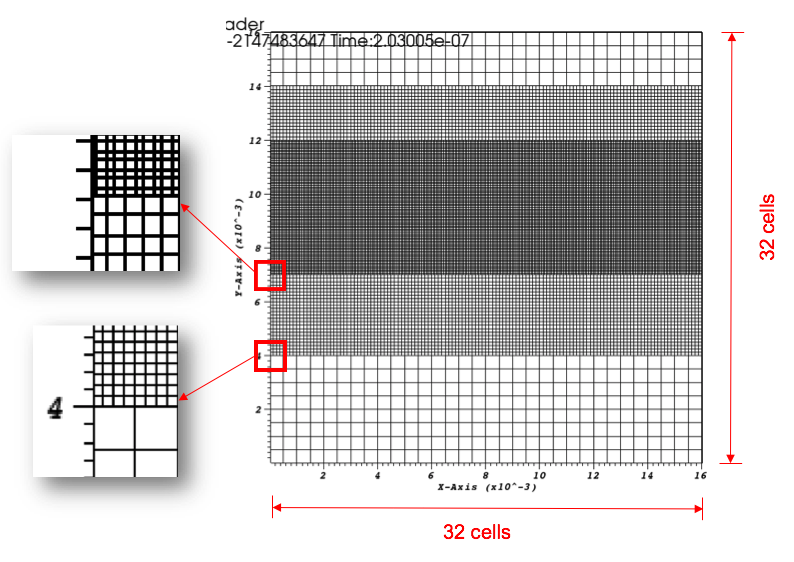
\includegraphics[width=8cm]{figs/AMR_resolution_explaination.png}
        \caption{AMR mesh grids outcome of the example configuration}
        \label{fig:AMR_resolution_explaination}
\end{figure}


\subsection{Results}
\subsubsection{Evaluation of different levels of refinement for different number of cores}
This experiment is first run on CAPER cluster, with a maximum of 128 cores, from level 1 to level 4 on 2, 4, 8, 16, 32, 64 and 128 cores. The execution time is recorded simply with the system tool ``time''.

\noindent
\textbf{Configuration}
\begin{table}[H]
\begin{center}
\begin{tabular}{|l|l|}
	\hline
	\textbf{Parameter} & \textbf{Value}\\ \hline
    Platform & CAPER and DELL cluster\\ 		\hline
    Number of cores & 2 to 128 quadratic growth\\
	\hline
    Level of refinement  & level 1 to level 4\\
    \hline
    Time step & 10\\
    \hline
    Time unit & Second\\
    \hline
\end{tabular}
\end{center}
\caption{Configuration for experiment of execution time of different levels of refinement under variety number of cores
}
\label{table:table_time_refinement}
\end{table}


\noindent
%\textbf{Result}
\begin{figure}[H]
	\centering
    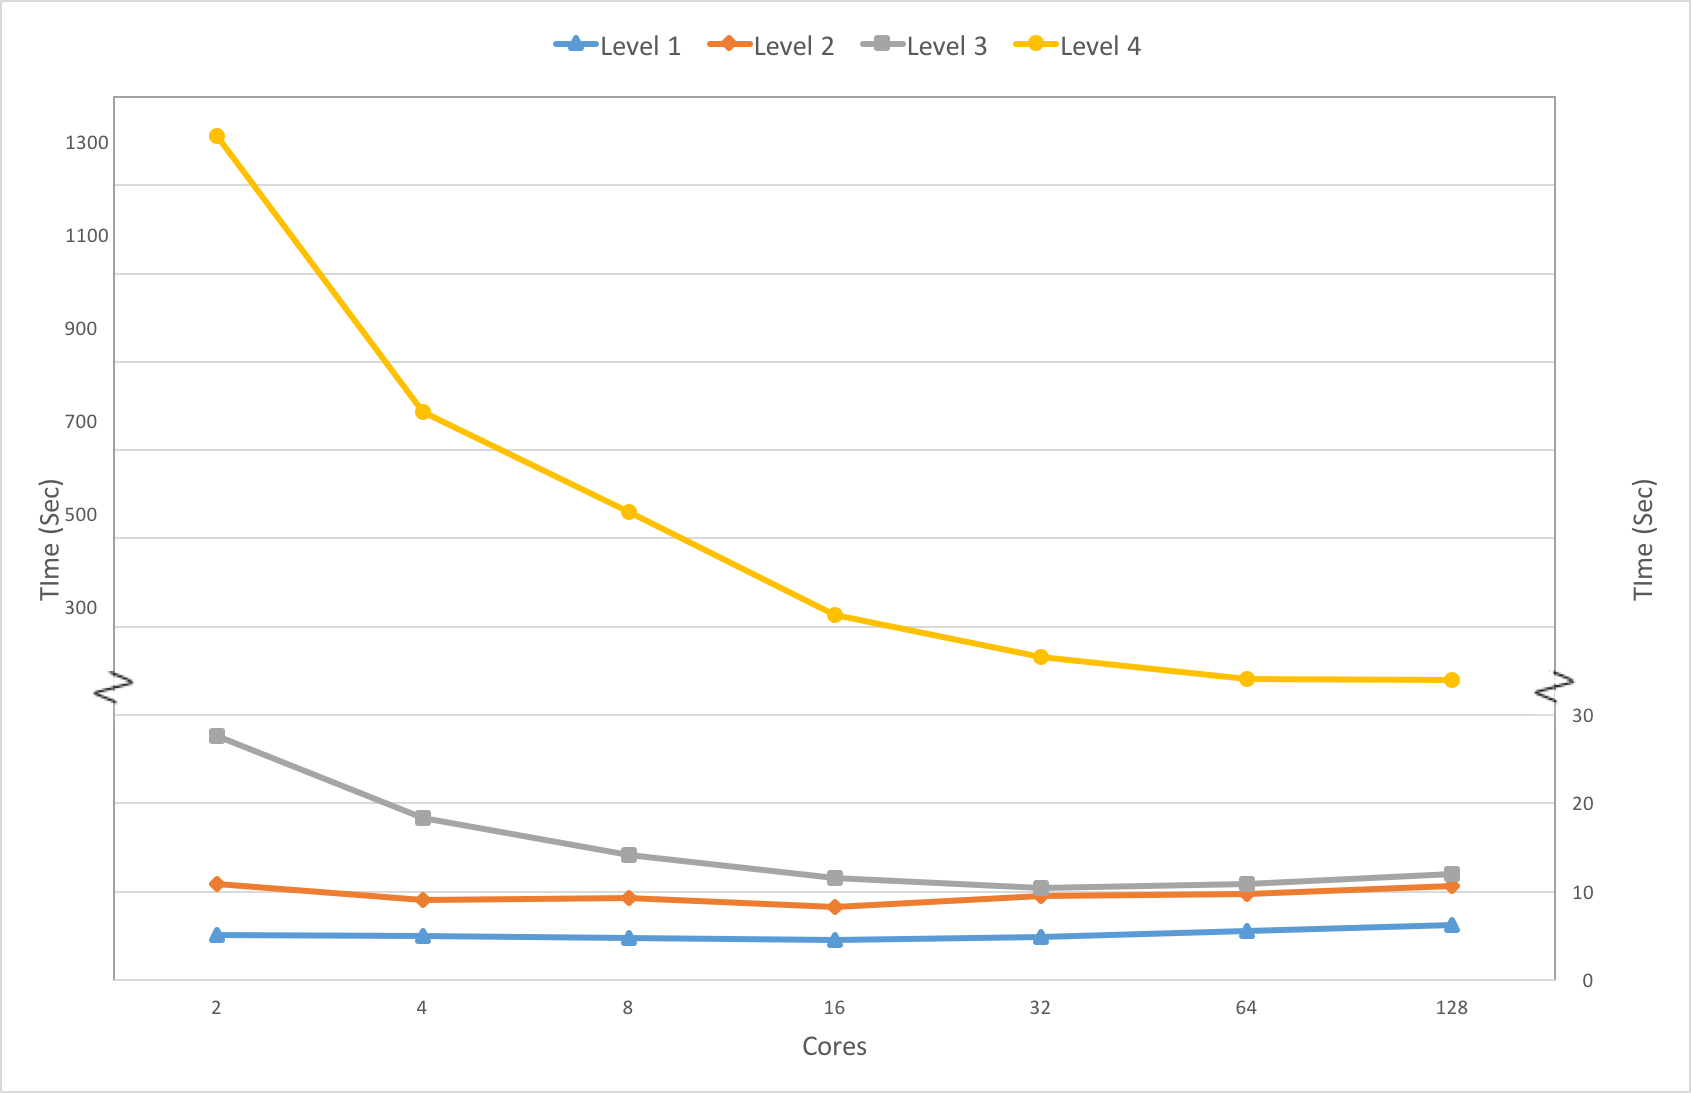
\includegraphics[width=8cm]{figs/CAPER_lev1-4_run_time_edited.jpg}
        \caption{Execution time of running different levels LMC on CAPER cluster through 2 to 128 cores. }
        \label{fig:executiontimeoncaper}
\end{figure}

\begin{figure}[H]
	\centering
    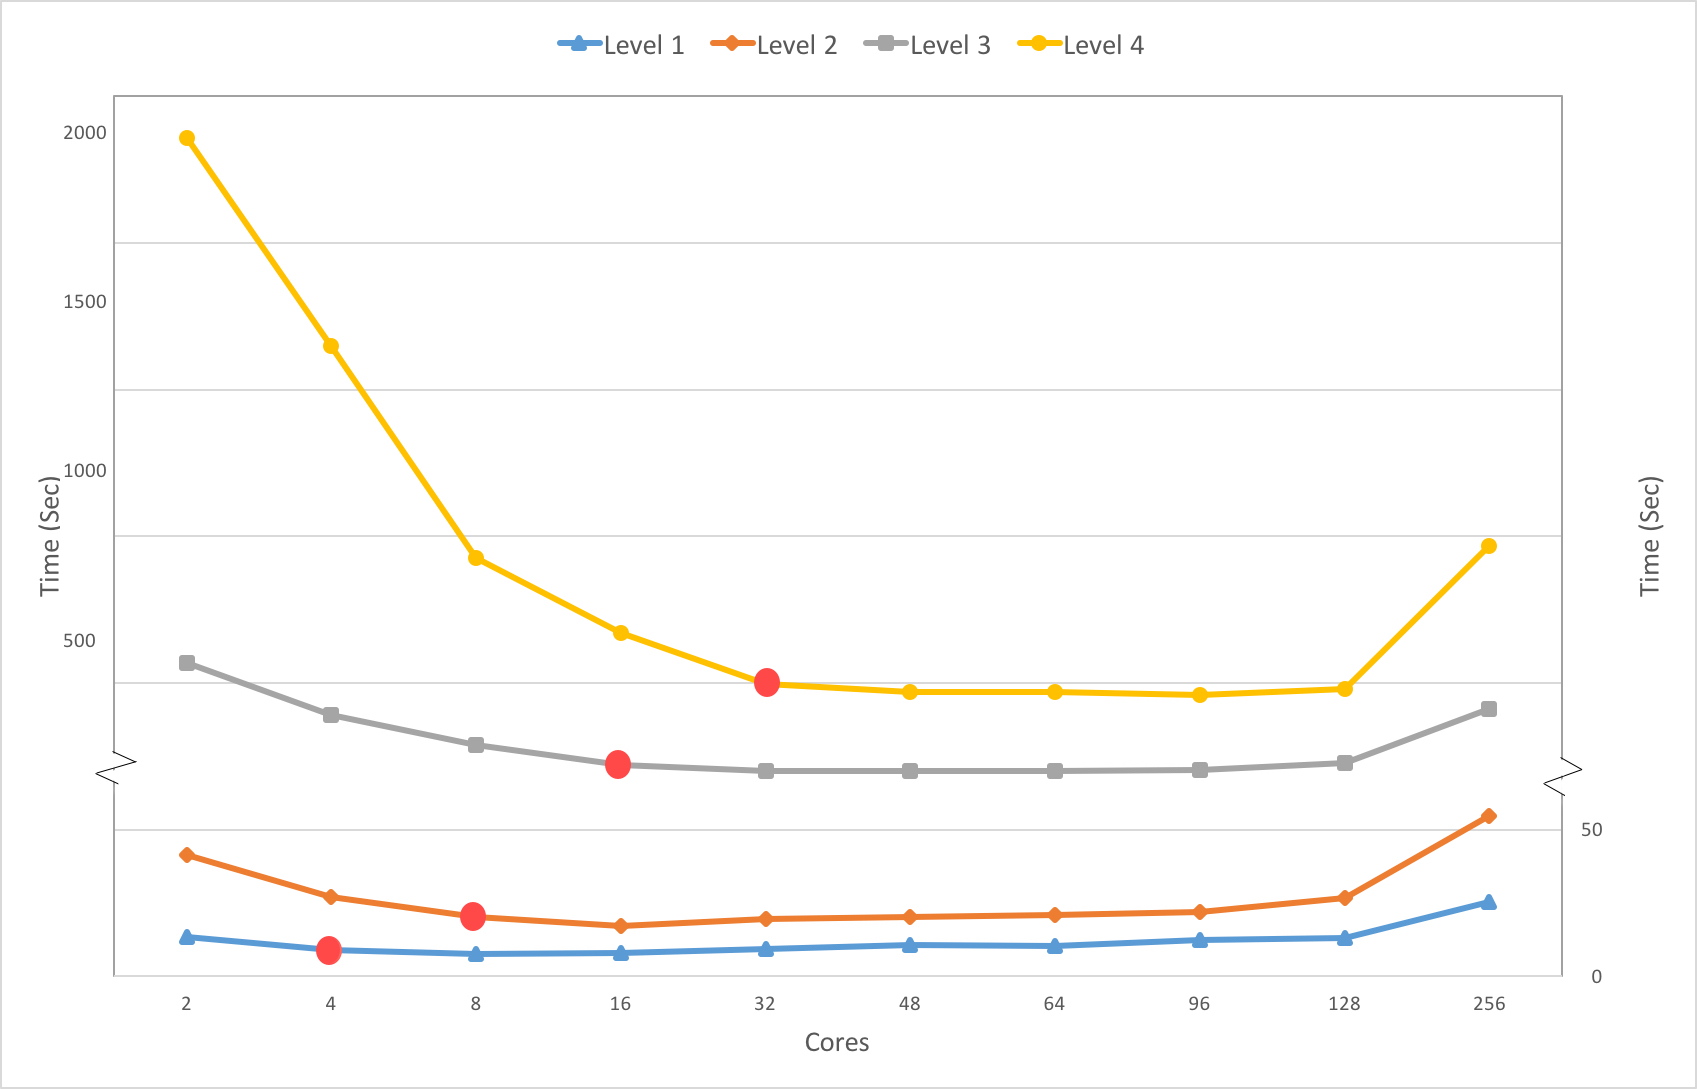
\includegraphics[width=8cm]{figs/Dell_lev1-4_run_time_edited.jpg}
        \caption{Execution time of running different levels LMC on DELL cluster through 2 to 256 cores. }
        \label{fig:executiontimeondell}
\end{figure}

%\noindent
%\textbf{Discussion}

The results of the first experiment using CAPER cluster are shown in Figure \ref{fig:executiontimeoncaper}. As can be clearly seen from the level 4 line, which is yellow line with solid dot maker, the more computing resource we use, the faster the execution is. Comparing these four lines, we can also notice that the slope is decreasing from level 4 to level 1, and then the lines go to a relative flat zoom. From this notice, we can see that heavier workload need more computational resources, but provisioning more resources do not bring any performance increase. In Figure \ref{fig:executiontimeoncaper} it can be seen from level 1 to level 3 lines that their tails are tilting a little bit, but level 4 line doesn’t have this trend. In order to show its trend more clearly, we ran this experiment on DELL cluster (256 cores cluster). The result is shown in Figure \ref{fig:executiontimeondell}. All levels' curve is like a ``U'', that tilt in the head and tile. From level 1 to level 4, the head turning point, which marked by red dot, are respectively 4, 8, 16 and 32 cores. Then they tend to get into a flat zoom, while under the 256 core, the execution time are all increase. From these two experiments we can conclude that, to achieve optimal running time, we need to configure appropriate number of processors to execute certain level of quality for the LMC program and using more processors does guarantee better performance.



\subsubsection{Evaluation of energy consumption of different levels of refinement under variety number of cores}
In this experiment, we are aim at exploring the energy consumption of running LMC with different level of refinement under multiple number of cores. 

%\noindent
%\textbf{Methodology}

Energy is the product of power and time, therefore, in this experiment, we need to measure the execution time and power respectively. To measure time, we still use Linux command TIME in the script file. And for the CPU power, we are using RAPL power meter to measure it. RAPL power meter is a sub-function of Intel Power Gadget program, which has been mentioned in previous background section. We are sampling power data every 0.5 second.

\noindent
\textbf{Configuration}
\begin{table}[H]
\begin{center}
\begin{tabular}{|l|l|}
	\hline
	\textbf{Parameter} & \textbf{Value}\\ \hline
    Platform & CAPER cluster\\ 		\hline
    Number of cores & 2 – 128 quadratic growth\\
	\hline
    Level of refinement  & level 1 to level 4\\
    \hline
    Time step & 10\\
    \hline
    Time unit & Second\\
    \hline
    Power measurement object & 8 nodes processors\\
    \hline
    RAPL sample rate & 2 Hz\\
    \hline
\end{tabular}
\end{center}
\caption{Configuration for experiment of power consumption of different levels of refinement under variety number of cores
}
\label{table:table_power_refinement}
\end{table}

\noindent
%\textbf{Result}
\begin{figure}[H]
	\centering
    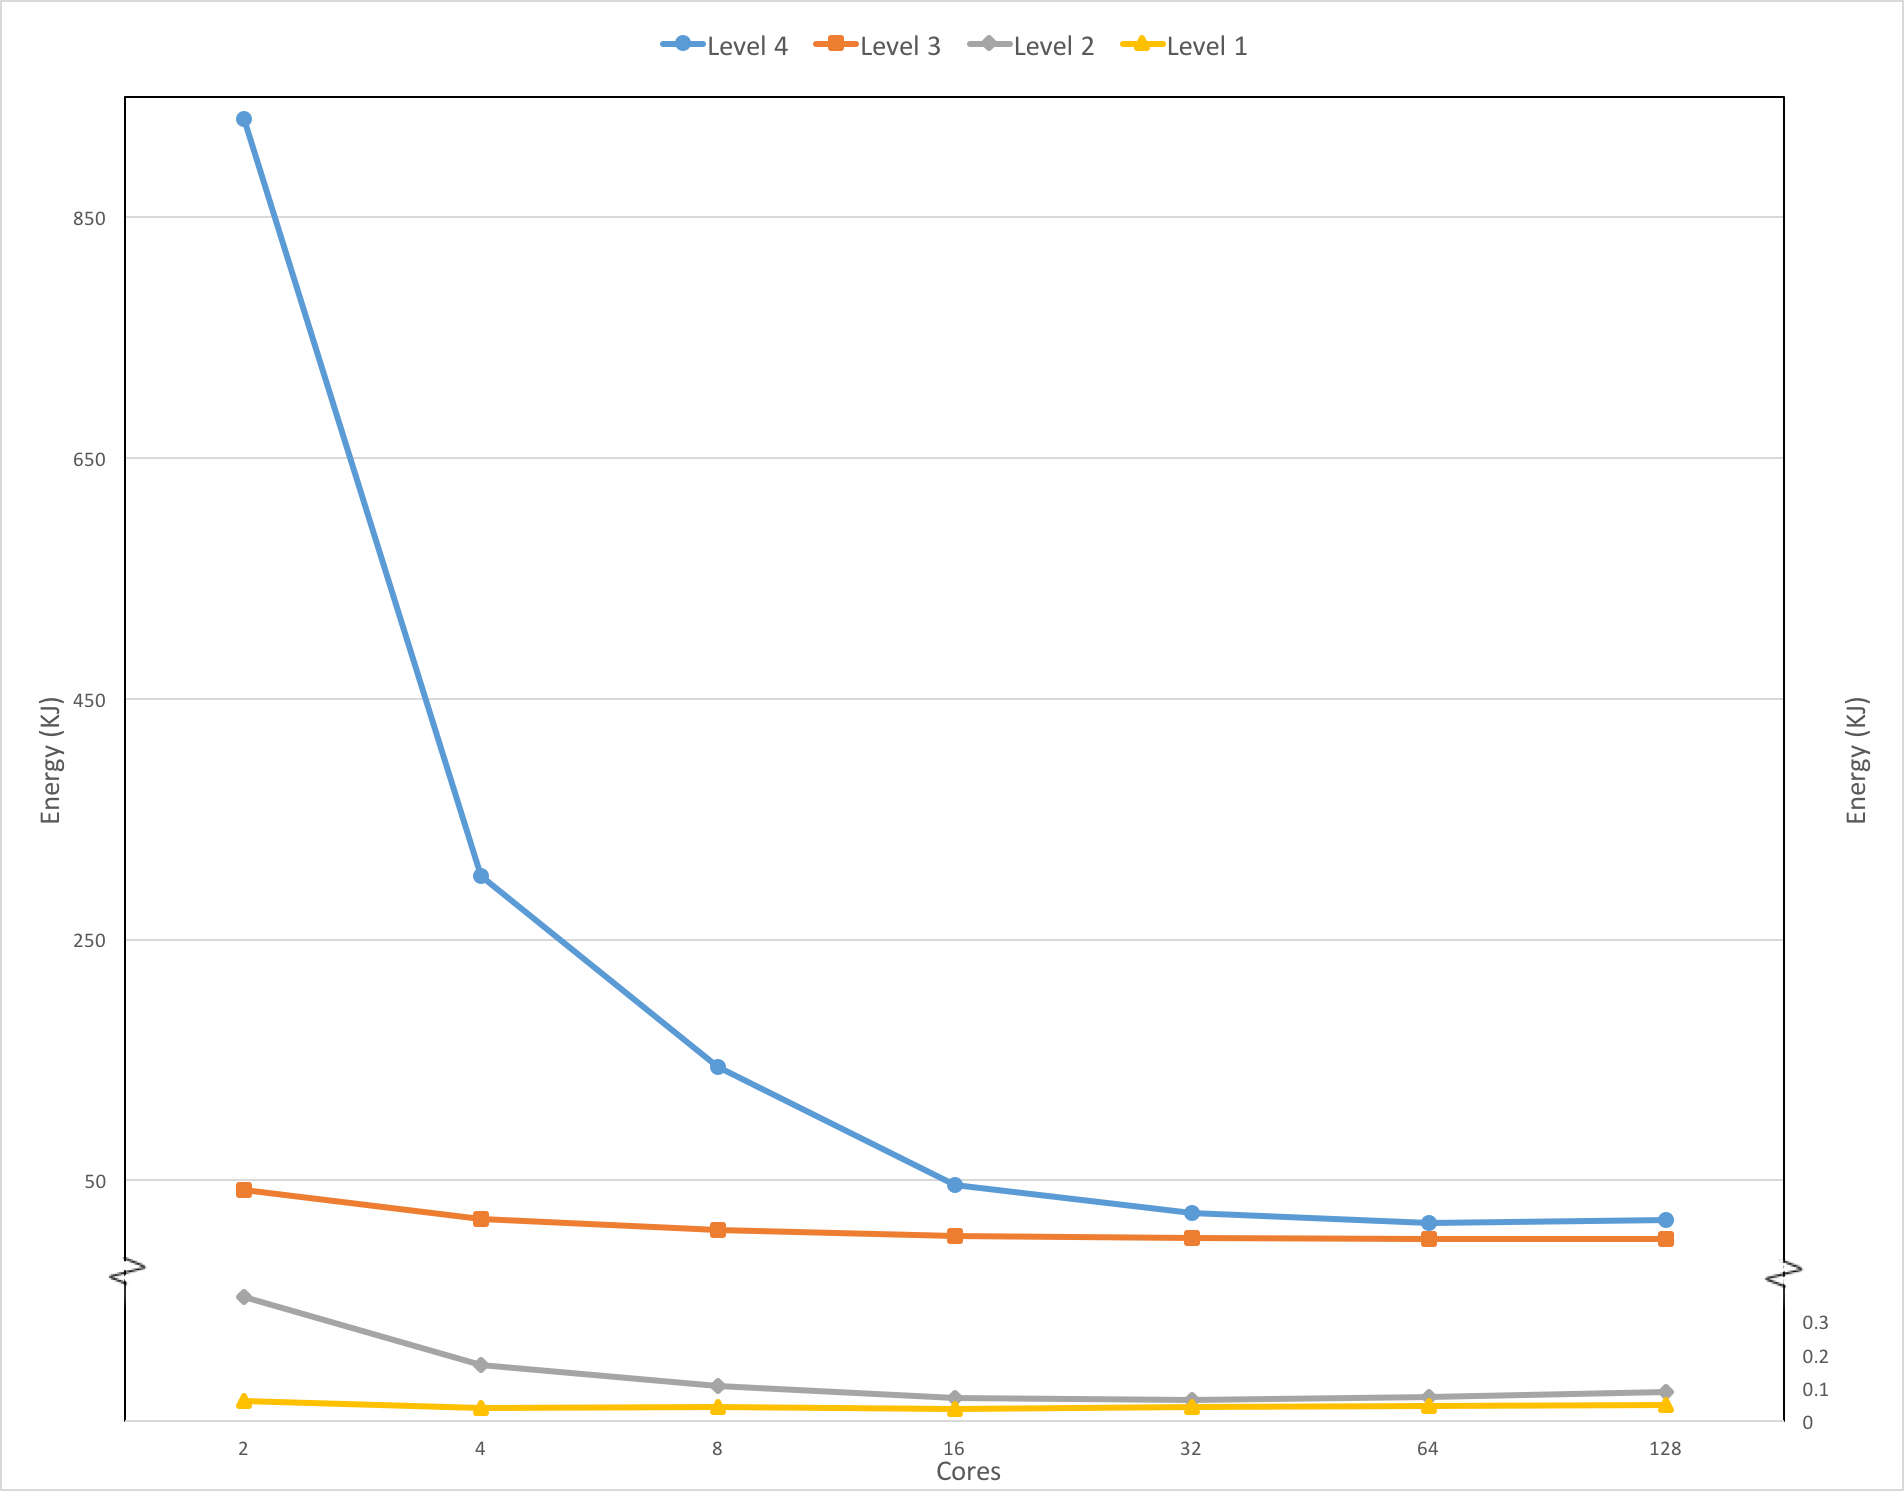
\includegraphics[width=8cm]{figs/CAPER_lev1-4_power_edited.jpg}
        \caption{Power consumption of different levels of refinement under different number of cores }
        \label{fig:powerconsumptioncaper}
\end{figure}

\noindent
%\textbf{Discussion}

Figure \ref{fig:powerconsumptioncaper} shows that there is a huge energy difference on the beginning of this curve. When running on 2 cores, the highest one (level 4) consumes almost 930 KJ while the lowest one (level 1) only take around 0.6 KJ. Since this experiment measure the all 8 node processors power status, the huge energy consumption of level 4 comes from the long execution time. It takes 1,314 seconds to run level 4 job while only 10 seconds to execute level 1. Most energy consumption comes from processors in idle state. But when assign appropriate processor resources to it, the curve reaches the flat zoom, the energy consumption difference is reasonable and stable. From this point of view, an appropriate number of cores for a certain workload is very crucial for energy consumption.



\subsubsection{Evaluation of the impact of RAPL power capping on LMC performance }
This experiment is aimed at studying the impact of power capping on LMC power-performance. And it would also give us a reference about the optimal power capping setting for different resolution levels. 


%\noindent
%\textbf{Methodology}

We use level 1 to level 4 in LMC as inputs to measure the time and power consumption. Since CAPER CPU power is 95W (Intel Xeon E5-2650 V2), in this experiment, we cap the CPU power to 25W, 35W, 45W, 55W, 65W, 75W, 85W, and 95W and record the package energy consumption (PKG) and execution time respectively. Package energy consumption is the energy used by the CPU chip itself including cores, caches and graphics, etc. 


\noindent
\textbf{Configuration}
\begin{table}[H]
\begin{center}
\begin{tabular}{|l|l|}
	\hline
	\textbf{Parameter} & \textbf{Value}\\ \hline
    Platform & CAPER cluster\\ 		\hline
    Number of cores & 64 cores\\
	\hline
    Level of refinement  & level 1 to level 4\\
    \hline
    Time step & 10\\
    \hline
    Time unit & Second\\
    \hline
    Power measurement object & 8 nodes processors\\
    \hline
    Power capping & 95W to 25W decrease by 10\\
    \hline
    RAPL sample rate & 2 Hz\\
    \hline
\end{tabular}
\end{center}
\caption{Configuration for experiment of exploring the affection of RAPL power capping on LMC performance 
}
\label{table:table_rapl_capping}
\end{table}

%\textbf{Power capping with RAPL}\\
We use Intel \textit{power\_gadget} tool to cap the power. To use it, we assign value to the parameter \textit{MY\_POWER\_LIMIT}, then compile and run it.
We use linux command line ``time'' to measure the execution time. The execution command line is provided as follows:
\begin{adjustwidth}{2cm}{4cm}
time mpirun -machinefile hostfile.txt -np 64 .\/LMC2d.Linux.g++.gfortran.SDC.MPI.ex inputfile amr.max\_lev=\#level
\end{adjustwidth}

For the power measurement, we also use the Intel \textit{power\_gadget} tool. When running it, it will give the real-time power consumption data every 0.5 second.



\noindent
%\textbf{Result}
\begin{figure}[H]
	\centering
    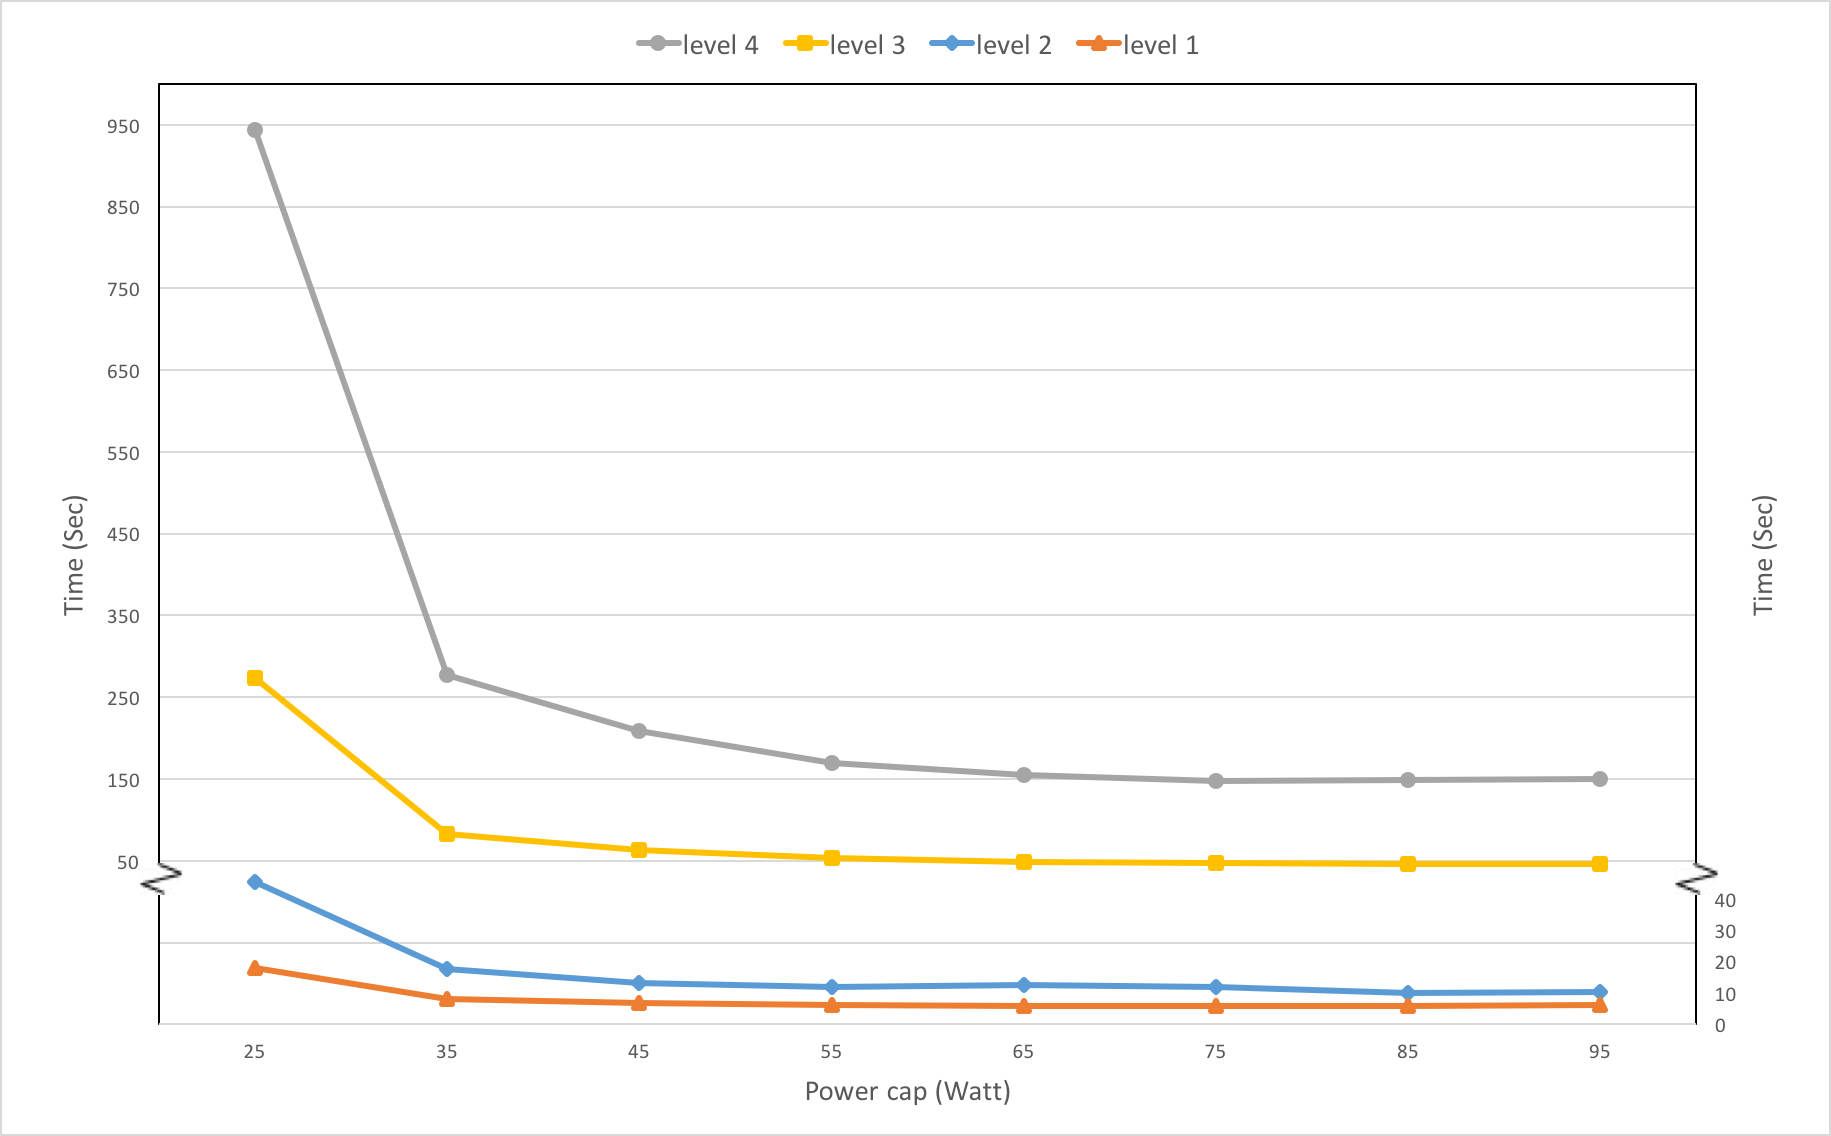
\includegraphics[width=8cm]{figs/CAPER_lev1-4_power_cap_time_edited.png}
        \caption{Relationship between different resolution of LMC and their execution time under different power capping levels}
        \label{fig:RAPLpowercaptime}
\end{figure}

\begin{figure}[H]
	\centering
    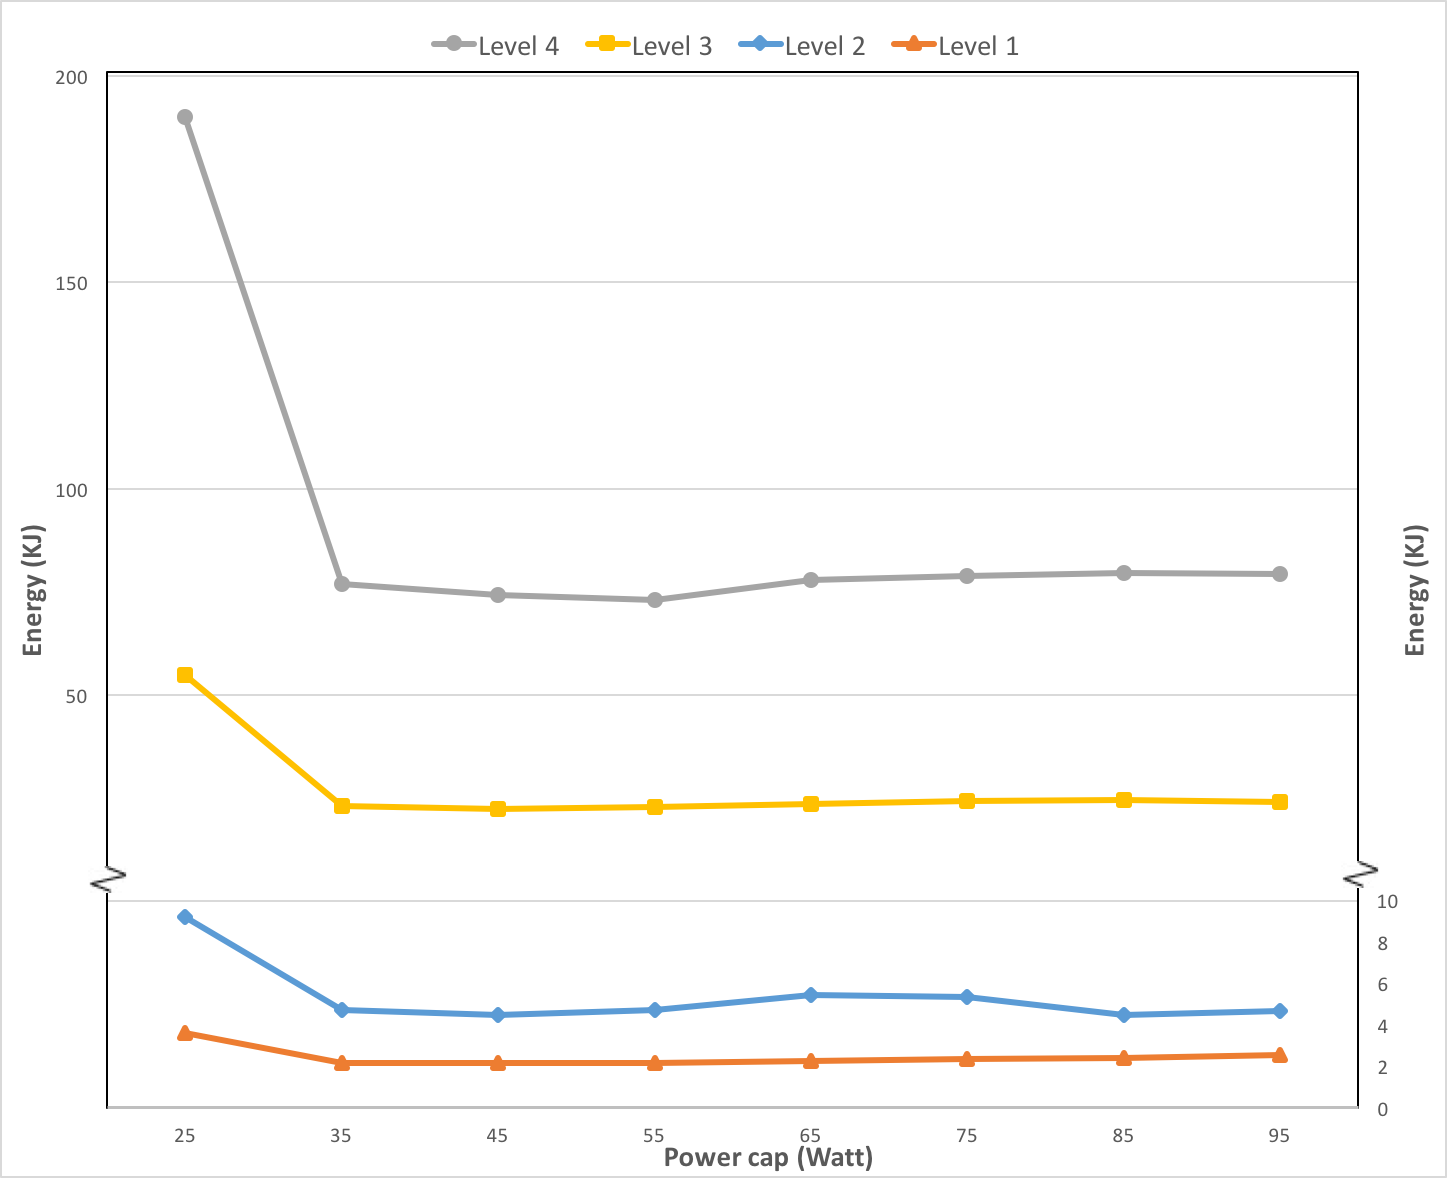
\includegraphics[width=8cm]{figs/CAPER_lev1-4_power_cap_energy_edited.png}
        \caption{Relationship between different resolution of LMC and the energy consumption under different power capping levels}
        \label{fig:RAPLpowercappower}
\end{figure}

\noindent
%\textbf{Discussion}

Figure presents the energy consumption result of executing level 1 to level 4 LMC program on certain number of cores under different power capping configurations. Those curves have the same pattern that sharply decreasing from 25 to 35 and becoming flat between 65 and 95. The lowest energy consumption is appearing when CPU power was capped to 45W to 55W. This can be explaining from execution data that without any CPU power capping, LMC program will boots CPU to 65W to 75W during execution whatever executing on how many cores. This also can be seem from the flat curve on segment 65W to 95W on each chart. Therefore, the advantage of power capping is working when CPU power down below 65W, and optimize between 45W to 55W. 



\subsubsection{Evaluation of power budget acquisition through power capping and resolution degradation}
The previous experiments have characterized the behavior of LMC. It can be concluded that the execution time will increase as the level of refinement/resolution increases or CPU power is capped down. Also, the energy consumption trend for different power caps and refinement levels is shown in Figure \ref{fig:Energy_consumption_trend}. The energy consumption presents the same trend as the execution time, i.e., LMC will consume more energy as the levels of refinement/resolution increase or capping down CPU power. The question here is how to use this characterization to create available power budget. We propose to combine these two factors, adjusting resolution and applying appropriate power capping, to get available power budget for running other tasks (e.g., checkpointing). 


\textbf{Configuration}
\begin{table}[H]
\begin{center}
\begin{tabular}{|l|l|}
	\hline
	\textbf{Parameter} & \textbf{Value}\\ \hline
    Platform & CAPER cluster\\ 		\hline
    Number of cores & 64 cores\\
	\hline
	Resolution & level 3 2 1\\
    \hline
    Time step & 10\\
    \hline
    Time unit & Second\\
    \hline
    Power measurement & RAPL meter\\
    \hline
    Power cap & RAPL\\
    \hline
\end{tabular}
\end{center}
\caption{Configuration for experiment of getting available power budget through power capping and resolution degradation
}
\label{table:table_tradeoff}
\end{table}



\begin{figure}[H]
	\centering
    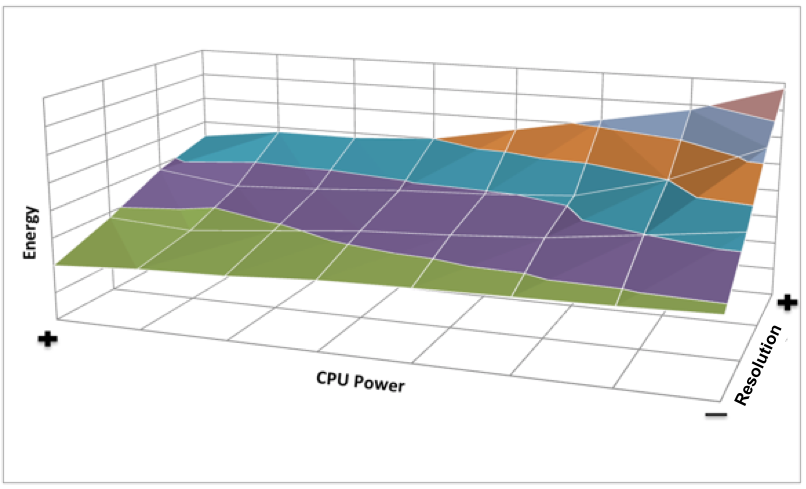
\includegraphics[width=8cm]{figs/Energy_consumption_trend.png}
        \caption{Energy consumption trend for different power caps and refinement levels}
        \label{fig:Energy_consumption_trend}
\end{figure}

\begin{figure}[H]
	\centering
    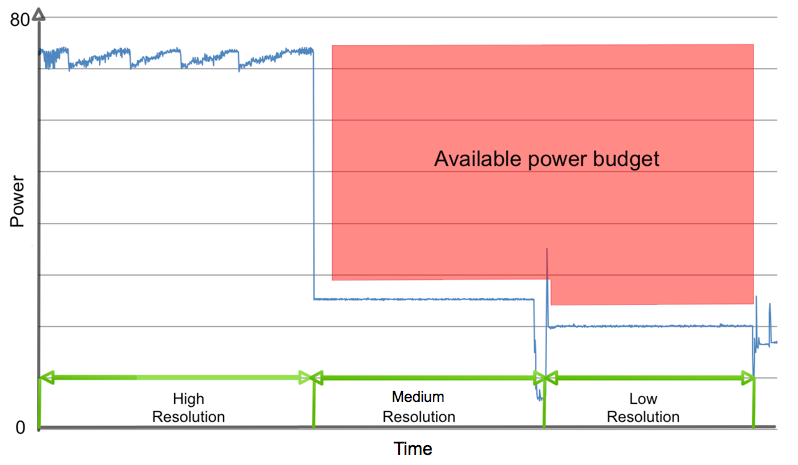
\includegraphics[width=8cm]{figs/Available_power_budget.png}
        \caption{Available power budget from applying resolution degradation and appropriate power capping}
        \label{fig:Available_power_budget}
\end{figure}


In previous Figure \ref{fig:LMCruntime}, we measured the power consumption of running LMC with different resolution. It shows that the execution time decreases when decreasing the resolution. Therefore, we apply appropriate power capping to the the medium and low resolution execution to make their execution equal the execution time in highest resolution. As shown in Figure \ref{fig:Available_power_budget}, the red region is the available power budget extracted from the total power budget. 



\subsubsection{Evaluation of power budget management}
We have tested the impact of power capping and level of refinement of LMC on the performance and energy consumption. We also observed the potential power saving from degrading resolution and implementing power capping. The goal of this experiment is being able to use power budgets opportunistically for running other tasks. In the experiment, we propose to use this power budget to do  checkpointing, which will increase the resilience and make the LMC program running more reliably. 

In this experiment, we are proposing to degrade LMC resolution and cap its running power, then use this power budget to do check pointing. However, there are some limitations due to the code characteristics: (i) we can not separate the checkpoint function from simulation program, and (ii) we can not dynamically control LMC resolution. 

%\textbf{Methodology}\\
To address these two issues, we use two LMC executions running alternatively on two set of nodes to emulate one execution dynamically adjusting resolution and doing checkpoint. Each set of nodes contains three nodes for execution. When the first execution start doing checkpoint then the second set start another execution with lower resolution. We focus on system level power consumption. 

We implement this using a flag to coordinate these two LMC executions. We've recompiled the first LMC set program to let it write flag when it start to do checkpoint, and the second LMC set keeps reading the flag to start running when the flag turn to be true. As shown in Figure \ref{fig:lev3withoutpowercap}, when the blue curve is the first instance (set 1) of LMC finishes its execution, it triggers the second instance (set 2), which is the orange curve. Once the second instance is completed the first one is triggered again and so on. By doing this, we can emulate a single LMC execution running and dynamically change the resolution while giving the available power budget for doing checkpoint.



\textbf{Configuration}
\begin{table}[H]
\begin{center}
\begin{tabular}{|l|l|}
	\hline
	\textbf{Parameter} & \textbf{Value}\\ \hline
    Platform & CAPER cluster\\ 		\hline
    Number of cores & 64 cores\\
	\hline
    Resolution & level 4 3\\
    \hline
    Time step & 10\\
    \hline
    Time unit & Second\\
    \hline
    Power measurement object & 3 nodes processors\\
    \hline
    Power cap & RAPL\\
    \hline
\end{tabular}
\end{center}
\caption{Configuration for experiment of exploring the power-performance tradeoffs 
}
\label{table:table_tradeoff}
\end{table}



\begin{figure}[H]
	\centering
    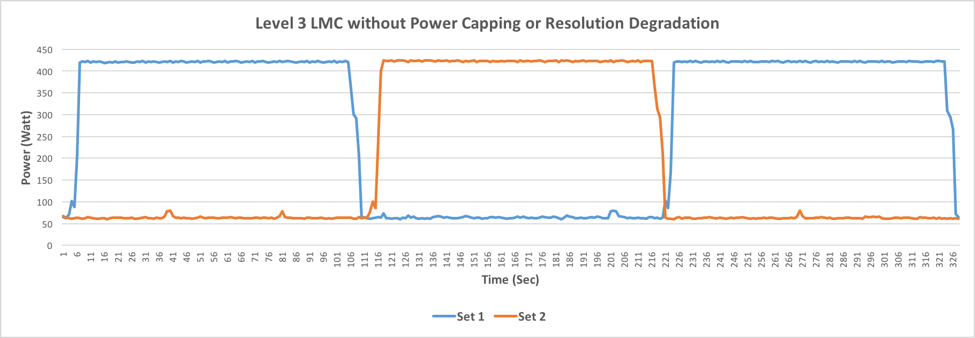
\includegraphics[width=8cm]{figs/lev3withoutpowercap.png}
        \caption{Level 3 LMC power consumption without power capping or resolution degradation}
        \label{fig:lev3withoutpowercap}
\end{figure}


\begin{figure}[H]
	\centering
    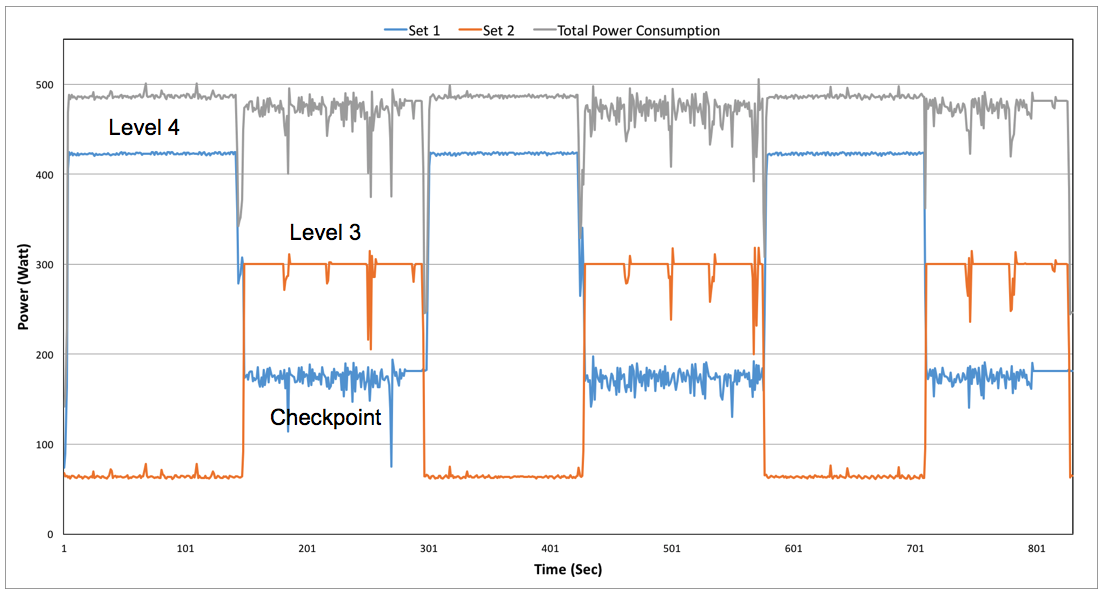
\includegraphics[width=8cm]{figs/LMCtradeoff.png}
        \caption{Level 4 LMC power consumption with power capping or resolution degradation}
        \label{fig:LMCtradeoff}
\end{figure}

In Figure \ref{fig:LMCtradeoff}, the blue curve is the set 1 running the high resolution LMC (level 4). Once it starts doing checkpointing, the set 2 (in orange curve) is triggered to run LMC at level 3. Configuring power capping appropriately, the total power consumption, which is shown in gray curve on the top, is kept constant. This means we successfully constraint the power budget of LMC to perform other tasks (i.e., checkpointing).






\section{Conclusion and future work}
In this work, we  have focused on studying the properties and exploring the performance, quality and power/energy tradeoffs of Low-Mach-Number Combustion (LMC) application which is based Adaptive Mesh Refinement (AMR) algorithm. The key contributions of this work are (1) we present an empirical evaluation of different configurations of application that gives insights into the energy-performance-quality tradeoff for this work, (2) we provided a comprehensive study of this LMC simulation performance, power and energy behavior, and (3) we propose a power-performance-quality tradeoff for this application, which can be used to better schedule power budgets across HPC systems.

Our current work investigates how to leverage these insights to implement a runtime to manage power budgets dynamically. Moreover, instead of trading-off with resolution, we also plan to explore the possibility of managing resources dynamically (e.g., cores) to manage power budgets. Future work also includes the management and scheduling of power budgets at whole system scale for assigning power budgets to other applications, not necessarily to the LMC workflow.




% conference papers do not normally have an appendix



% trigger a \newpage just before the given reference
% number - used to balance the columns on the last page
% adjust value as needed - may need to be readjusted if
% the document is modified later
%\IEEEtriggeratref{8}
% The "triggered" command can be changed if desired:
%\IEEEtriggercmd{\enlargethispage{-5in}}

% references section

% can use a bibliography generated by BibTeX as a .bbl file
% BibTeX documentation can be easily obtained at:
% http://www.ctan.org/tex-archive/biblio/bibtex/contrib/doc/
% The IEEEtran BibTeX style support page is at:
% http://www.michaelshell.org/tex/ieeetran/bibtex/
%\bibliographystyle{IEEEtran}
% argument is your BibTeX string definitions and bibliography database(s)
%\bibliography{IEEEabrv,../bib/paper}
%
% <OR> manually copy in the resultant .bbl file
% set second argument of \begin to the number of references
% (used to reserve space for the reference number labels box)
% \begin{thebibliography}{1}

% \bibitem{IEEEhowto:kopka}
% H.~Kopka and P.~W. Daly, \emph{A Guide to \LaTeX}, 3rd~ed.\hskip 1em plus
%   0.5em minus 0.4em\relax Harlow, England: Addison-Wesley, 1999.

% \end{thebibliography}

\bibliographystyle{IEEEtran}
\bibliography{references}

% that's all folks
\end{document}


